\begin{figure}[ht!]
\begin{center}
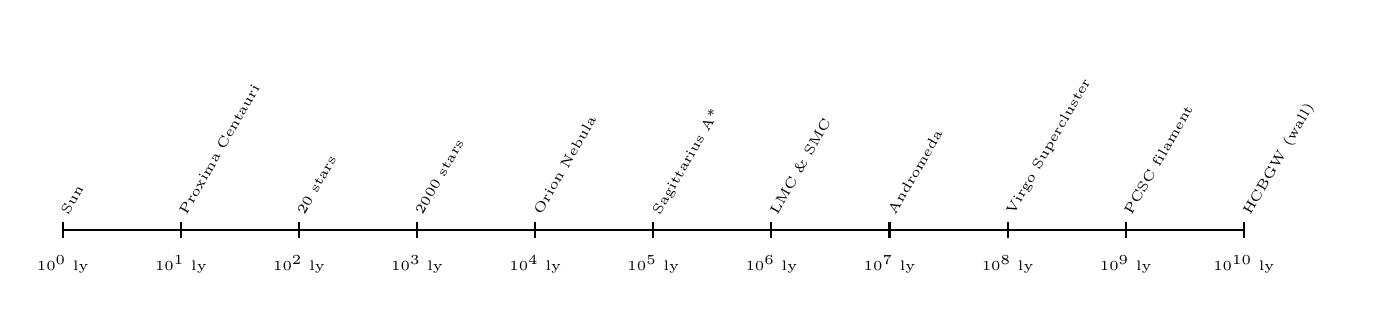
\begin{tikzpicture}
    % Parameters
    \def\n{10}
    \def\length{15}
    \def\spacing{\length/\n}

    % Labels array
    \def\labels{{"Sun", "Proxima Centauri", "20 stars", "2000 stars", "Orion Nebula", "Sagittarius A*", 
                 "LMC \& SMC", "Andromeda", "Virgo Supercluster", 
                 "PCSC filament", "HCBGW (wall)"}}

    % Draw base line
    \draw[thick] (0,0) -- (\length,0);

    % Draw tick marks, numbers and rotated labels
    \foreach \i in {0,...,10} {
        \pgfmathsetmacro{\x}{\i*\spacing}
        \draw[thick] (\x,0.1) -- (\x,-0.1); % Tick
        \node[below, font=\tiny] at (\x, -0.2) {$10^{\i}$ ly};      % Number
        
        % Multi-line labels with a 2-line approach for long labels
        \node[above, font=\tiny, text width=2.5cm, rotate=60, anchor=north west] at (\x-0.2,+0.2) 
            {\pgfmathparse{\labels[\i]}\pgfmathresult}; % Label
    }
\end{tikzpicture}
\caption{Cosmic distances span from nearby stars to the largest known structures in the universe, measured on scales of light-years, typically up to the order of 10. Each label represents either the distance to a notable astronomical object or the size of a vast cosmic region. The diameter of the observable universe is roughly 93 billion light-years, which is nearly the order of 11.}
\end{center}
\end{figure}

